\documentclass[twoside]{book}

% Packages required by doxygen
\usepackage{fixltx2e}
\usepackage{calc}
\usepackage{doxygen}
\usepackage[export]{adjustbox} % also loads graphicx
\usepackage{graphicx}
\usepackage[utf8]{inputenc}
\usepackage{makeidx}
\usepackage{multicol}
\usepackage{multirow}
\PassOptionsToPackage{warn}{textcomp}
\usepackage{textcomp}
\usepackage[nointegrals]{wasysym}
\usepackage[table]{xcolor}

% Font selection
\usepackage[T1]{fontenc}
\usepackage[scaled=.90]{helvet}
\usepackage{courier}
\usepackage{amssymb}
\usepackage{sectsty}
\renewcommand{\familydefault}{\sfdefault}
\allsectionsfont{%
  \fontseries{bc}\selectfont%
  \color{darkgray}%
}
\renewcommand{\DoxyLabelFont}{%
  \fontseries{bc}\selectfont%
  \color{darkgray}%
}
\newcommand{\+}{\discretionary{\mbox{\scriptsize$\hookleftarrow$}}{}{}}

% Page & text layout
\usepackage{geometry}
\geometry{%
  a4paper,%
  top=2.5cm,%
  bottom=2.5cm,%
  left=2.5cm,%
  right=2.5cm%
}
\tolerance=750
\hfuzz=15pt
\hbadness=750
\setlength{\emergencystretch}{15pt}
\setlength{\parindent}{0cm}
\setlength{\parskip}{3ex plus 2ex minus 2ex}
\makeatletter
\renewcommand{\paragraph}{%
  \@startsection{paragraph}{4}{0ex}{-1.0ex}{1.0ex}{%
    \normalfont\normalsize\bfseries\SS@parafont%
  }%
}
\renewcommand{\subparagraph}{%
  \@startsection{subparagraph}{5}{0ex}{-1.0ex}{1.0ex}{%
    \normalfont\normalsize\bfseries\SS@subparafont%
  }%
}
\makeatother

% Headers & footers
\usepackage{fancyhdr}
\pagestyle{fancyplain}
\fancyhead[LE]{\fancyplain{}{\bfseries\thepage}}
\fancyhead[CE]{\fancyplain{}{}}
\fancyhead[RE]{\fancyplain{}{\bfseries\leftmark}}
\fancyhead[LO]{\fancyplain{}{\bfseries\rightmark}}
\fancyhead[CO]{\fancyplain{}{}}
\fancyhead[RO]{\fancyplain{}{\bfseries\thepage}}
\fancyfoot[LE]{\fancyplain{}{}}
\fancyfoot[CE]{\fancyplain{}{}}
\fancyfoot[RE]{\fancyplain{}{\bfseries\scriptsize Generated by Doxygen }}
\fancyfoot[LO]{\fancyplain{}{\bfseries\scriptsize Generated by Doxygen }}
\fancyfoot[CO]{\fancyplain{}{}}
\fancyfoot[RO]{\fancyplain{}{}}
\renewcommand{\footrulewidth}{0.4pt}
\renewcommand{\chaptermark}[1]{%
  \markboth{#1}{}%
}
\renewcommand{\sectionmark}[1]{%
  \markright{\thesection\ #1}%
}

% Indices & bibliography
\usepackage{natbib}
\usepackage[titles]{tocloft}
\setcounter{tocdepth}{3}
\setcounter{secnumdepth}{5}
\makeindex

% Hyperlinks (required, but should be loaded last)
\usepackage{ifpdf}
\ifpdf
  \usepackage[pdftex,pagebackref=true]{hyperref}
\else
  \usepackage[ps2pdf,pagebackref=true]{hyperref}
\fi
\hypersetup{%
  colorlinks=true,%
  linkcolor=blue,%
  citecolor=blue,%
  unicode%
}

% Custom commands
\newcommand{\clearemptydoublepage}{%
  \newpage{\pagestyle{empty}\cleardoublepage}%
}

\usepackage{caption}
\captionsetup{labelsep=space,justification=centering,font={bf},singlelinecheck=off,skip=4pt,position=top}

%===== C O N T E N T S =====

\begin{document}

% Titlepage & ToC
\hypersetup{pageanchor=false,
             bookmarksnumbered=true,
             pdfencoding=unicode
            }
\pagenumbering{alph}
\begin{titlepage}
\vspace*{7cm}
\begin{center}%
{\Large My Project \\[1ex]\large 1 }\\
\vspace*{1cm}
{\large Generated by Doxygen 1.8.13}\\
\end{center}
\end{titlepage}
\clearemptydoublepage
\pagenumbering{roman}
\tableofcontents
\clearemptydoublepage
\pagenumbering{arabic}
\hypersetup{pageanchor=true}

%--- Begin generated contents ---
\chapter{Data Structure Index}
\section{Class List}
Here are the classes, structs, unions and interfaces with brief descriptions\+:\begin{DoxyCompactList}
\item\contentsline{section}{\hyperlink{class_a_v_l_tree}{A\+V\+L\+Tree} \\*Class for A\+VL Tree }{\pageref{class_a_v_l_tree}}{}
\item\contentsline{section}{\hyperlink{structnode}{node} }{\pageref{structnode}}{}
\item\contentsline{section}{\hyperlink{class_node}{Node} }{\pageref{class_node}}{}
\item\contentsline{section}{\hyperlink{struct_r_b_t_node}{R\+B\+T\+Node} \\*\hyperlink{struct_r_b_t_node}{R\+B\+T\+Node} for red black tree }{\pageref{struct_r_b_t_node}}{}
\item\contentsline{section}{\hyperlink{class_r_b_tree}{R\+B\+Tree} \\*Class to represent Red-\/\+Black Tree }{\pageref{class_r_b_tree}}{}
\end{DoxyCompactList}

\chapter{File Index}
\section{File List}
Here is a list of all files with brief descriptions\+:\begin{DoxyCompactList}
\item\contentsline{section}{/home/kavya/\+Desktop/csn261\+\_\+lab\+\_\+assignment1/q1/code/\hyperlink{q1_8c}{q1.\+c} }{\pageref{q1_8c}}{}
\end{DoxyCompactList}

\chapter{Data Structure Documentation}
\hypertarget{struct_q_node}{}\section{Q\+Node Struct Reference}
\label{struct_q_node}\index{Q\+Node@{Q\+Node}}


\hyperlink{struct_q_node}{Q\+Node} for storing unused\+Rolls.  




Collaboration diagram for Q\+Node\+:
\nopagebreak
\begin{figure}[H]
\begin{center}
\leavevmode
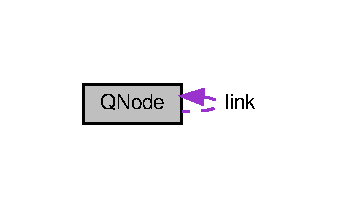
\includegraphics[width=164pt]{struct_q_node__coll__graph}
\end{center}
\end{figure}
\subsection*{Data Fields}
\begin{DoxyCompactItemize}
\item 
int \hyperlink{struct_q_node_a9eab91667db4d35c7231dcddf7b89a76}{data}
\item 
struct \hyperlink{struct_q_node}{Q\+Node} $\ast$ \hyperlink{struct_q_node_aeb974434dabad67698cafa3278f141a0}{link}
\end{DoxyCompactItemize}


\subsection{Detailed Description}
\hyperlink{struct_q_node}{Q\+Node} for storing unused\+Rolls. 

Definition at line 29 of file q1.\+c.



\subsection{Field Documentation}
\mbox{\Hypertarget{struct_q_node_a9eab91667db4d35c7231dcddf7b89a76}\label{struct_q_node_a9eab91667db4d35c7231dcddf7b89a76}} 
\index{Q\+Node@{Q\+Node}!data@{data}}
\index{data@{data}!Q\+Node@{Q\+Node}}
\subsubsection{\texorpdfstring{data}{data}}
{\footnotesize\ttfamily int data}



Definition at line 30 of file q1.\+c.

\mbox{\Hypertarget{struct_q_node_aeb974434dabad67698cafa3278f141a0}\label{struct_q_node_aeb974434dabad67698cafa3278f141a0}} 
\index{Q\+Node@{Q\+Node}!link@{link}}
\index{link@{link}!Q\+Node@{Q\+Node}}
\subsubsection{\texorpdfstring{link}{link}}
{\footnotesize\ttfamily struct \hyperlink{struct_q_node}{Q\+Node}$\ast$ link}



Definition at line 31 of file q1.\+c.



The documentation for this struct was generated from the following file\+:\begin{DoxyCompactItemize}
\item 
/home/kavya/\+Desktop/csn261\+\_\+lab\+\_\+assignment1/q1/code/\hyperlink{q1_8c}{q1.\+c}\end{DoxyCompactItemize}

\hypertarget{struct_student}{}\section{Student Struct Reference}
\label{struct_student}\index{Student@{Student}}


student nodes storing Roll,Name,Address,D\+OB and Phone number.  




Collaboration diagram for Student\+:
\nopagebreak
\begin{figure}[H]
\begin{center}
\leavevmode
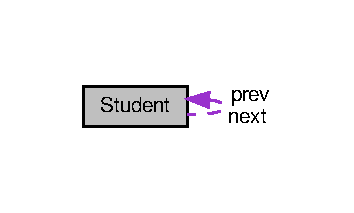
\includegraphics[width=170pt]{struct_student__coll__graph}
\end{center}
\end{figure}
\subsection*{Data Fields}
\begin{DoxyCompactItemize}
\item 
int \hyperlink{struct_student_abf08303c7c1c86949317530985b66f65}{Roll}
\item 
char \hyperlink{struct_student_a6b7a07c8ee9c9f38664df19619d58228}{Name} \mbox{[}100\mbox{]}
\item 
char \hyperlink{struct_student_ac8b69a306e0bda4dbd3ff7195b193577}{Address} \mbox{[}100\mbox{]}
\item 
char \hyperlink{struct_student_ac7f4f37722482a16f12dc314d0d1360f}{D\+OB} \mbox{[}20\mbox{]}
\item 
long long int \hyperlink{struct_student_a097ef0dc0739c67e89950dec9f3c1446}{Phone}
\item 
struct \hyperlink{struct_student}{Student} $\ast$ \hyperlink{struct_student_a6a280e6c00fedbc058905a9b06e2bc91}{next}
\item 
struct \hyperlink{struct_student}{Student} $\ast$ \hyperlink{struct_student_acccaf7a7261d26814e081163b772728f}{prev}
\end{DoxyCompactItemize}


\subsection{Detailed Description}
student nodes storing Roll,Name,Address,D\+OB and Phone number. 

Definition at line 17 of file q1.\+c.



\subsection{Field Documentation}
\mbox{\Hypertarget{struct_student_ac8b69a306e0bda4dbd3ff7195b193577}\label{struct_student_ac8b69a306e0bda4dbd3ff7195b193577}} 
\index{Student@{Student}!Address@{Address}}
\index{Address@{Address}!Student@{Student}}
\subsubsection{\texorpdfstring{Address}{Address}}
{\footnotesize\ttfamily char Address\mbox{[}100\mbox{]}}



Definition at line 19 of file q1.\+c.

\mbox{\Hypertarget{struct_student_ac7f4f37722482a16f12dc314d0d1360f}\label{struct_student_ac7f4f37722482a16f12dc314d0d1360f}} 
\index{Student@{Student}!D\+OB@{D\+OB}}
\index{D\+OB@{D\+OB}!Student@{Student}}
\subsubsection{\texorpdfstring{D\+OB}{DOB}}
{\footnotesize\ttfamily char D\+OB\mbox{[}20\mbox{]}}



Definition at line 19 of file q1.\+c.

\mbox{\Hypertarget{struct_student_a6b7a07c8ee9c9f38664df19619d58228}\label{struct_student_a6b7a07c8ee9c9f38664df19619d58228}} 
\index{Student@{Student}!Name@{Name}}
\index{Name@{Name}!Student@{Student}}
\subsubsection{\texorpdfstring{Name}{Name}}
{\footnotesize\ttfamily char Name\mbox{[}100\mbox{]}}



Definition at line 19 of file q1.\+c.

\mbox{\Hypertarget{struct_student_a6a280e6c00fedbc058905a9b06e2bc91}\label{struct_student_a6a280e6c00fedbc058905a9b06e2bc91}} 
\index{Student@{Student}!next@{next}}
\index{next@{next}!Student@{Student}}
\subsubsection{\texorpdfstring{next}{next}}
{\footnotesize\ttfamily struct \hyperlink{struct_student}{Student}$\ast$ next}



Definition at line 21 of file q1.\+c.

\mbox{\Hypertarget{struct_student_a097ef0dc0739c67e89950dec9f3c1446}\label{struct_student_a097ef0dc0739c67e89950dec9f3c1446}} 
\index{Student@{Student}!Phone@{Phone}}
\index{Phone@{Phone}!Student@{Student}}
\subsubsection{\texorpdfstring{Phone}{Phone}}
{\footnotesize\ttfamily long long int Phone}



Definition at line 20 of file q1.\+c.

\mbox{\Hypertarget{struct_student_acccaf7a7261d26814e081163b772728f}\label{struct_student_acccaf7a7261d26814e081163b772728f}} 
\index{Student@{Student}!prev@{prev}}
\index{prev@{prev}!Student@{Student}}
\subsubsection{\texorpdfstring{prev}{prev}}
{\footnotesize\ttfamily struct \hyperlink{struct_student}{Student} $\ast$ prev}



Definition at line 21 of file q1.\+c.

\mbox{\Hypertarget{struct_student_abf08303c7c1c86949317530985b66f65}\label{struct_student_abf08303c7c1c86949317530985b66f65}} 
\index{Student@{Student}!Roll@{Roll}}
\index{Roll@{Roll}!Student@{Student}}
\subsubsection{\texorpdfstring{Roll}{Roll}}
{\footnotesize\ttfamily int Roll}



Definition at line 18 of file q1.\+c.



The documentation for this struct was generated from the following file\+:\begin{DoxyCompactItemize}
\item 
/home/kavya/\+Desktop/csn261\+\_\+lab\+\_\+assignment1/q1/code/\hyperlink{q1_8c}{q1.\+c}\end{DoxyCompactItemize}

\chapter{File Documentation}
\hypertarget{q1_8c}{}\section{/home/kavya/\+Desktop/csn261\+\_\+lab\+\_\+assignment1/q1/code/q1.c File Reference}
\label{q1_8c}\index{/home/kavya/\+Desktop/csn261\+\_\+lab\+\_\+assignment1/q1/code/q1.\+c@{/home/kavya/\+Desktop/csn261\+\_\+lab\+\_\+assignment1/q1/code/q1.\+c}}
{\ttfamily \#include $<$stdio.\+h$>$}\newline
{\ttfamily \#include $<$stdlib.\+h$>$}\newline
{\ttfamily \#include $<$string.\+h$>$}\newline
{\ttfamily \#include $<$time.\+h$>$}\newline
Include dependency graph for q1.\+c\+:
\nopagebreak
\begin{figure}[H]
\begin{center}
\leavevmode
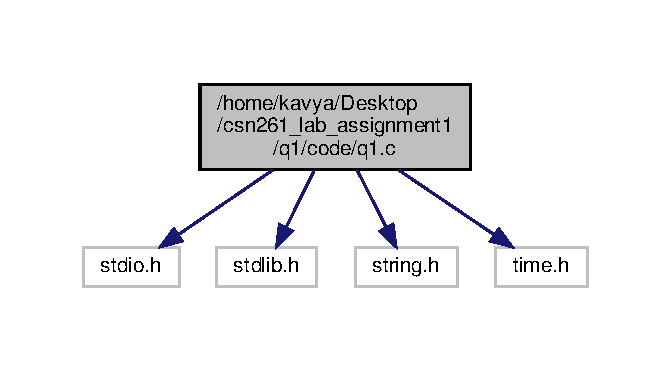
\includegraphics[width=322pt]{q1_8c__incl}
\end{center}
\end{figure}
\subsection*{Data Structures}
\begin{DoxyCompactItemize}
\item 
struct \hyperlink{struct_student}{Student}
\begin{DoxyCompactList}\small\item\em student nodes storing Roll,Name,Address,D\+OB and Phone number. \end{DoxyCompactList}\item 
struct \hyperlink{struct_q_node}{Q\+Node}
\begin{DoxyCompactList}\small\item\em \hyperlink{struct_q_node}{Q\+Node} for storing unused\+Rolls. \end{DoxyCompactList}\end{DoxyCompactItemize}
\subsection*{Functions}
\begin{DoxyCompactItemize}
\item 
void \hyperlink{q1_8c_a28040132a3b8ad1dbacdf2a7b5456324}{enqueue} (int d)
\begin{DoxyCompactList}\small\item\em enqueue data into the queue for unused\+Rolls \end{DoxyCompactList}\item 
int \hyperlink{q1_8c_ad6e0da35e82ee741ee4e9779fdf9e1c9}{dequeue} ()
\begin{DoxyCompactList}\small\item\em dequeue data from the queue for unused\+Rolls \end{DoxyCompactList}\item 
struct \hyperlink{struct_student}{Student} $\ast$ \hyperlink{q1_8c_a0c9e567a874149bbd3bafac57055228d}{search} (int roll)
\item 
void \hyperlink{q1_8c_a35c71ffe4242840e71e590fd7460bfb2}{insert\+Student} (char nm\mbox{[}$\,$\mbox{]}, char dob\mbox{[}$\,$\mbox{]}, char adrs\mbox{[}$\,$\mbox{]}, long long int phone)
\item 
struct \hyperlink{struct_student}{Student} $\ast$ \hyperlink{q1_8c_aadd4e680f1f42d39a5ef8d217cba9e9f}{delete} (int roll)
\item 
void \hyperlink{q1_8c_a6862f05c55f3e2b4fc7483bbe8c5e66e}{modify} (int roll, char nm\mbox{[}$\,$\mbox{]}, char dob\mbox{[}$\,$\mbox{]}, char adrs\mbox{[}$\,$\mbox{]}, long long int phone)
\item 
void \hyperlink{q1_8c_a1fde8665b00c0d8b37581447a7dcb959}{print} (struct \hyperlink{struct_student}{Student} $\ast$n)
\item 
void \hyperlink{q1_8c_ac3d6b1c1e40ddae8a7b4273be5d7c091}{swap} (struct \hyperlink{struct_student}{Student} $\ast$s1, struct \hyperlink{struct_student}{Student} $\ast$s2)
\item 
void \hyperlink{q1_8c_a47fdc9eea42b6975cdc835bb2e08810e}{sort} ()
\item 
void \hyperlink{q1_8c_a2145130bf1a181011d026cf0fc97e1e4}{remove\+Char} (char $\ast$s, int c)
\item 
long long int \hyperlink{q1_8c_a0d7446f3b40f9b93b5def4c6453cdd14}{Convert\+Char\+To\+Long} (char $\ast$p\+Src)
\item 
void \hyperlink{q1_8c_a9a146e54485452a350f21d5c32f8a96b}{get\+Data} (char data\mbox{[}$\,$\mbox{]})
\item 
void \hyperlink{q1_8c_ab1703367762abc1490e00dcd5ccb29bc}{read\+Data} ()
\item 
void \hyperlink{q1_8c_a63e83e1746a7d77e0dd4a27af9b51e96}{insert} (int num)
\item 
int \hyperlink{q1_8c_ae66f6b31b5ad750f1fe042a706a4e3d4}{main} ()
\end{DoxyCompactItemize}
\subsection*{Variables}
\begin{DoxyCompactItemize}
\item 
struct \hyperlink{struct_student}{Student} $\ast$ \hyperlink{q1_8c_aa26c266dac077132d25008e29b6bb1c5}{first} = N\+U\+LL
\begin{DoxyCompactList}\small\item\em first and last Nodes pointing to front and rear of doubly-\/linked-\/list \end{DoxyCompactList}\item 
struct \hyperlink{struct_student}{Student} $\ast$ \hyperlink{q1_8c_aa8dff5b0cd1a0f043d232bc6b42bfef9}{last} =N\+U\+LL
\item 
int \hyperlink{q1_8c_a7347196987a9a7a7abf12cdaf9e54f49}{roll\+Count} =100
\begin{DoxyCompactList}\small\item\em containing the current roll count at each instant \end{DoxyCompactList}\item 
struct \hyperlink{struct_q_node}{Q\+Node} $\ast$ \hyperlink{q1_8c_a74f2bd32b733faa4cb558a4055478a72}{Qfront} =N\+U\+LL
\begin{DoxyCompactList}\small\item\em Qfront and Qrear are the pointers to front and rear of the queue. \end{DoxyCompactList}\item 
struct \hyperlink{struct_q_node}{Q\+Node} $\ast$ \hyperlink{q1_8c_a8ce9ad364c967e211fae5a2ede256e4e}{Qrear} =N\+U\+LL
\end{DoxyCompactItemize}


\subsection{Function Documentation}
\mbox{\Hypertarget{q1_8c_a0d7446f3b40f9b93b5def4c6453cdd14}\label{q1_8c_a0d7446f3b40f9b93b5def4c6453cdd14}} 
\index{q1.\+c@{q1.\+c}!Convert\+Char\+To\+Long@{Convert\+Char\+To\+Long}}
\index{Convert\+Char\+To\+Long@{Convert\+Char\+To\+Long}!q1.\+c@{q1.\+c}}
\subsubsection{\texorpdfstring{Convert\+Char\+To\+Long()}{ConvertCharToLong()}}
{\footnotesize\ttfamily long long int Convert\+Char\+To\+Long (\begin{DoxyParamCaption}\item[{char $\ast$}]{p\+Src }\end{DoxyParamCaption})}



Definition at line 246 of file q1.\+c.

\mbox{\Hypertarget{q1_8c_aadd4e680f1f42d39a5ef8d217cba9e9f}\label{q1_8c_aadd4e680f1f42d39a5ef8d217cba9e9f}} 
\index{q1.\+c@{q1.\+c}!delete@{delete}}
\index{delete@{delete}!q1.\+c@{q1.\+c}}
\subsubsection{\texorpdfstring{delete()}{delete()}}
{\footnotesize\ttfamily struct \hyperlink{struct_student}{Student}$\ast$ delete (\begin{DoxyParamCaption}\item[{int}]{roll }\end{DoxyParamCaption})}

This method will be used to perform deletion of student with given Roll. \begin{DoxyAuthor}{Author}
Kavya Barnwal 
\end{DoxyAuthor}

\begin{DoxyParams}{Parameters}
{\em roll} & used to search in Data\+Base \\
\hline
\end{DoxyParams}
\begin{DoxyDate}{Date}
31/07/2019 
\end{DoxyDate}


Definition at line 126 of file q1.\+c.

\mbox{\Hypertarget{q1_8c_ad6e0da35e82ee741ee4e9779fdf9e1c9}\label{q1_8c_ad6e0da35e82ee741ee4e9779fdf9e1c9}} 
\index{q1.\+c@{q1.\+c}!dequeue@{dequeue}}
\index{dequeue@{dequeue}!q1.\+c@{q1.\+c}}
\subsubsection{\texorpdfstring{dequeue()}{dequeue()}}
{\footnotesize\ttfamily int dequeue (\begin{DoxyParamCaption}{ }\end{DoxyParamCaption})}



dequeue data from the queue for unused\+Rolls 



Definition at line 49 of file q1.\+c.

\mbox{\Hypertarget{q1_8c_a28040132a3b8ad1dbacdf2a7b5456324}\label{q1_8c_a28040132a3b8ad1dbacdf2a7b5456324}} 
\index{q1.\+c@{q1.\+c}!enqueue@{enqueue}}
\index{enqueue@{enqueue}!q1.\+c@{q1.\+c}}
\subsubsection{\texorpdfstring{enqueue()}{enqueue()}}
{\footnotesize\ttfamily void enqueue (\begin{DoxyParamCaption}\item[{int}]{d }\end{DoxyParamCaption})}



enqueue data into the queue for unused\+Rolls 



Definition at line 36 of file q1.\+c.

\mbox{\Hypertarget{q1_8c_a9a146e54485452a350f21d5c32f8a96b}\label{q1_8c_a9a146e54485452a350f21d5c32f8a96b}} 
\index{q1.\+c@{q1.\+c}!get\+Data@{get\+Data}}
\index{get\+Data@{get\+Data}!q1.\+c@{q1.\+c}}
\subsubsection{\texorpdfstring{get\+Data()}{getData()}}
{\footnotesize\ttfamily void get\+Data (\begin{DoxyParamCaption}\item[{char}]{data\mbox{[}$\,$\mbox{]} }\end{DoxyParamCaption})}



Definition at line 255 of file q1.\+c.

\mbox{\Hypertarget{q1_8c_a63e83e1746a7d77e0dd4a27af9b51e96}\label{q1_8c_a63e83e1746a7d77e0dd4a27af9b51e96}} 
\index{q1.\+c@{q1.\+c}!insert@{insert}}
\index{insert@{insert}!q1.\+c@{q1.\+c}}
\subsubsection{\texorpdfstring{insert()}{insert()}}
{\footnotesize\ttfamily void insert (\begin{DoxyParamCaption}\item[{int}]{num }\end{DoxyParamCaption})}

This method will be used to perform insertion of student with given number. \begin{DoxyAuthor}{Author}
Kavya Barnwal 
\end{DoxyAuthor}

\begin{DoxyParams}{Parameters}
{\em num} & representing the (row-\/1) to be inserted \\
\hline
\end{DoxyParams}
\begin{DoxyDate}{Date}
31/07/2019 
\end{DoxyDate}


Definition at line 305 of file q1.\+c.

\mbox{\Hypertarget{q1_8c_a35c71ffe4242840e71e590fd7460bfb2}\label{q1_8c_a35c71ffe4242840e71e590fd7460bfb2}} 
\index{q1.\+c@{q1.\+c}!insert\+Student@{insert\+Student}}
\index{insert\+Student@{insert\+Student}!q1.\+c@{q1.\+c}}
\subsubsection{\texorpdfstring{insert\+Student()}{insertStudent()}}
{\footnotesize\ttfamily void insert\+Student (\begin{DoxyParamCaption}\item[{char}]{nm\mbox{[}$\,$\mbox{]},  }\item[{char}]{dob\mbox{[}$\,$\mbox{]},  }\item[{char}]{adrs\mbox{[}$\,$\mbox{]},  }\item[{long long int}]{phone }\end{DoxyParamCaption})}

This method will be used to inser\+Student with given details except Roll. \begin{DoxyAuthor}{Author}
Kavya Barnwal 
\end{DoxyAuthor}

\begin{DoxyParams}{Parameters}
{\em name,dob,addrs,phone} & required details of sudents \\
\hline
\end{DoxyParams}
\begin{DoxyDate}{Date}
31/07/2019 
\end{DoxyDate}


Definition at line 94 of file q1.\+c.

\mbox{\Hypertarget{q1_8c_ae66f6b31b5ad750f1fe042a706a4e3d4}\label{q1_8c_ae66f6b31b5ad750f1fe042a706a4e3d4}} 
\index{q1.\+c@{q1.\+c}!main@{main}}
\index{main@{main}!q1.\+c@{q1.\+c}}
\subsubsection{\texorpdfstring{main()}{main()}}
{\footnotesize\ttfamily int main (\begin{DoxyParamCaption}{ }\end{DoxyParamCaption})}



Definition at line 321 of file q1.\+c.

\mbox{\Hypertarget{q1_8c_a6862f05c55f3e2b4fc7483bbe8c5e66e}\label{q1_8c_a6862f05c55f3e2b4fc7483bbe8c5e66e}} 
\index{q1.\+c@{q1.\+c}!modify@{modify}}
\index{modify@{modify}!q1.\+c@{q1.\+c}}
\subsubsection{\texorpdfstring{modify()}{modify()}}
{\footnotesize\ttfamily void modify (\begin{DoxyParamCaption}\item[{int}]{roll,  }\item[{char}]{nm\mbox{[}$\,$\mbox{]},  }\item[{char}]{dob\mbox{[}$\,$\mbox{]},  }\item[{char}]{adrs\mbox{[}$\,$\mbox{]},  }\item[{long long int}]{phone }\end{DoxyParamCaption})}

This method will be used to modify details of student excpept Roll. \begin{DoxyAuthor}{Author}
Kavya Barnwal 
\end{DoxyAuthor}

\begin{DoxyParams}{Parameters}
{\em roll} & used to search in Data\+Base, nm,dob,adrs,phone to be updated. \\
\hline
\end{DoxyParams}
\begin{DoxyDate}{Date}
31/07/2019 
\end{DoxyDate}


Definition at line 166 of file q1.\+c.

\mbox{\Hypertarget{q1_8c_a1fde8665b00c0d8b37581447a7dcb959}\label{q1_8c_a1fde8665b00c0d8b37581447a7dcb959}} 
\index{q1.\+c@{q1.\+c}!print@{print}}
\index{print@{print}!q1.\+c@{q1.\+c}}
\subsubsection{\texorpdfstring{print()}{print()}}
{\footnotesize\ttfamily void print (\begin{DoxyParamCaption}\item[{struct \hyperlink{struct_student}{Student} $\ast$}]{n }\end{DoxyParamCaption})}

This method will be used to print the list of all students. \begin{DoxyAuthor}{Author}
Kavya Barnwal 
\end{DoxyAuthor}

\begin{DoxyParams}{Parameters}
{\em student,head} & of the Doubly-\/linked-\/list of students \\
\hline
\end{DoxyParams}
\begin{DoxyDate}{Date}
31/07/2019 
\end{DoxyDate}


Definition at line 182 of file q1.\+c.

\mbox{\Hypertarget{q1_8c_ab1703367762abc1490e00dcd5ccb29bc}\label{q1_8c_ab1703367762abc1490e00dcd5ccb29bc}} 
\index{q1.\+c@{q1.\+c}!read\+Data@{read\+Data}}
\index{read\+Data@{read\+Data}!q1.\+c@{q1.\+c}}
\subsubsection{\texorpdfstring{read\+Data()}{readData()}}
{\footnotesize\ttfamily void read\+Data (\begin{DoxyParamCaption}{ }\end{DoxyParamCaption})}

This method will be used to read the complete data in Student.\+csv file(all students). \begin{DoxyAuthor}{Author}
Kavya Barnwal 
\end{DoxyAuthor}
\begin{DoxyDate}{Date}
31/07/2019 
\end{DoxyDate}


Definition at line 286 of file q1.\+c.

\mbox{\Hypertarget{q1_8c_a2145130bf1a181011d026cf0fc97e1e4}\label{q1_8c_a2145130bf1a181011d026cf0fc97e1e4}} 
\index{q1.\+c@{q1.\+c}!remove\+Char@{remove\+Char}}
\index{remove\+Char@{remove\+Char}!q1.\+c@{q1.\+c}}
\subsubsection{\texorpdfstring{remove\+Char()}{removeChar()}}
{\footnotesize\ttfamily void remove\+Char (\begin{DoxyParamCaption}\item[{char $\ast$}]{s,  }\item[{int}]{c }\end{DoxyParamCaption})}



Definition at line 237 of file q1.\+c.

\mbox{\Hypertarget{q1_8c_a0c9e567a874149bbd3bafac57055228d}\label{q1_8c_a0c9e567a874149bbd3bafac57055228d}} 
\index{q1.\+c@{q1.\+c}!search@{search}}
\index{search@{search}!q1.\+c@{q1.\+c}}
\subsubsection{\texorpdfstring{search()}{search()}}
{\footnotesize\ttfamily struct \hyperlink{struct_student}{Student}$\ast$ search (\begin{DoxyParamCaption}\item[{int}]{roll }\end{DoxyParamCaption})}

This method will be used to search the student with given Roll. \begin{DoxyAuthor}{Author}
Kavya Barnwal 
\end{DoxyAuthor}

\begin{DoxyParams}{Parameters}
{\em roll} & used to search in Data\+Base \\
\hline
\end{DoxyParams}
\begin{DoxyDate}{Date}
31/07/2019 
\end{DoxyDate}


Definition at line 76 of file q1.\+c.

\mbox{\Hypertarget{q1_8c_a47fdc9eea42b6975cdc835bb2e08810e}\label{q1_8c_a47fdc9eea42b6975cdc835bb2e08810e}} 
\index{q1.\+c@{q1.\+c}!sort@{sort}}
\index{sort@{sort}!q1.\+c@{q1.\+c}}
\subsubsection{\texorpdfstring{sort()}{sort()}}
{\footnotesize\ttfamily void sort (\begin{DoxyParamCaption}{ }\end{DoxyParamCaption})}

This method will be used to perform sorting by name. \begin{DoxyAuthor}{Author}
Kavya Barnwal 
\end{DoxyAuthor}
\begin{DoxyDate}{Date}
31/07/2019 
\end{DoxyDate}


Definition at line 223 of file q1.\+c.

\mbox{\Hypertarget{q1_8c_ac3d6b1c1e40ddae8a7b4273be5d7c091}\label{q1_8c_ac3d6b1c1e40ddae8a7b4273be5d7c091}} 
\index{q1.\+c@{q1.\+c}!swap@{swap}}
\index{swap@{swap}!q1.\+c@{q1.\+c}}
\subsubsection{\texorpdfstring{swap()}{swap()}}
{\footnotesize\ttfamily void swap (\begin{DoxyParamCaption}\item[{struct \hyperlink{struct_student}{Student} $\ast$}]{s1,  }\item[{struct \hyperlink{struct_student}{Student} $\ast$}]{s2 }\end{DoxyParamCaption})}

This method will be used to perform swapping of details of two students. \begin{DoxyAuthor}{Author}
Kavya Barnwal 
\end{DoxyAuthor}

\begin{DoxyParams}{Parameters}
{\em s1,s2} & to be swapped \\
\hline
\end{DoxyParams}
\begin{DoxyDate}{Date}
31/07/2019 
\end{DoxyDate}


Definition at line 197 of file q1.\+c.



\subsection{Variable Documentation}
\mbox{\Hypertarget{q1_8c_aa26c266dac077132d25008e29b6bb1c5}\label{q1_8c_aa26c266dac077132d25008e29b6bb1c5}} 
\index{q1.\+c@{q1.\+c}!first@{first}}
\index{first@{first}!q1.\+c@{q1.\+c}}
\subsubsection{\texorpdfstring{first}{first}}
{\footnotesize\ttfamily struct \hyperlink{struct_student}{Student}$\ast$ first = N\+U\+LL}



first and last Nodes pointing to front and rear of doubly-\/linked-\/list 



Definition at line 24 of file q1.\+c.

\mbox{\Hypertarget{q1_8c_aa8dff5b0cd1a0f043d232bc6b42bfef9}\label{q1_8c_aa8dff5b0cd1a0f043d232bc6b42bfef9}} 
\index{q1.\+c@{q1.\+c}!last@{last}}
\index{last@{last}!q1.\+c@{q1.\+c}}
\subsubsection{\texorpdfstring{last}{last}}
{\footnotesize\ttfamily struct \hyperlink{struct_student}{Student} $\ast$ last =N\+U\+LL}



Definition at line 24 of file q1.\+c.

\mbox{\Hypertarget{q1_8c_a74f2bd32b733faa4cb558a4055478a72}\label{q1_8c_a74f2bd32b733faa4cb558a4055478a72}} 
\index{q1.\+c@{q1.\+c}!Qfront@{Qfront}}
\index{Qfront@{Qfront}!q1.\+c@{q1.\+c}}
\subsubsection{\texorpdfstring{Qfront}{Qfront}}
{\footnotesize\ttfamily struct \hyperlink{struct_q_node}{Q\+Node}$\ast$ Qfront =N\+U\+LL}



Qfront and Qrear are the pointers to front and rear of the queue. 



Definition at line 34 of file q1.\+c.

\mbox{\Hypertarget{q1_8c_a8ce9ad364c967e211fae5a2ede256e4e}\label{q1_8c_a8ce9ad364c967e211fae5a2ede256e4e}} 
\index{q1.\+c@{q1.\+c}!Qrear@{Qrear}}
\index{Qrear@{Qrear}!q1.\+c@{q1.\+c}}
\subsubsection{\texorpdfstring{Qrear}{Qrear}}
{\footnotesize\ttfamily struct \hyperlink{struct_q_node}{Q\+Node} $\ast$ Qrear =N\+U\+LL}



Definition at line 34 of file q1.\+c.

\mbox{\Hypertarget{q1_8c_a7347196987a9a7a7abf12cdaf9e54f49}\label{q1_8c_a7347196987a9a7a7abf12cdaf9e54f49}} 
\index{q1.\+c@{q1.\+c}!roll\+Count@{roll\+Count}}
\index{roll\+Count@{roll\+Count}!q1.\+c@{q1.\+c}}
\subsubsection{\texorpdfstring{roll\+Count}{rollCount}}
{\footnotesize\ttfamily int roll\+Count =100}



containing the current roll count at each instant 



Definition at line 26 of file q1.\+c.


%--- End generated contents ---

% Index
\backmatter
\newpage
\phantomsection
\clearemptydoublepage
\addcontentsline{toc}{chapter}{Index}
\printindex

\end{document}
